%%%%%%%%%%%%%%%%%%%%%%%%%%%%%%%%%%%%%%%%%%%%%%%%%%%%%%%%%%%%%%%%%%%%%%%%%%%%%%%
\subsection{Introduction}
%%%%%%%%%%%%%%%%%%%%%%%%%%%%%%%%%%%%%%%%%%%%%%%%%%%%%%%%%%%%%%%%%%%%%%%%%%%%%%%
\begin{frame}
 \begin{colorblock}{blue}{lightblue}{ }
    \Large \textbf{Introduction}
  \end{colorblock}
\end{frame}

\begin{frame}
\frametitle{Introduction and Motivations}
\begin{itemize}
	\item {\bf Clusters of commodity servers are a major computing platform}
	\begin{itemize}
		\item Modern Internet Services
		\item Data-intensive applications
	\end{itemize}
	\item {\bf New computing {\it Frameworks} developed to ``program the cluster''}
	\begin{itemize}
		\item Hadoop MapReduce, Apache Spark, Microsoft Dryad
		\item Pregel, Storm, ...
		\item and many more
	\end{itemize}
	\item {\bf No {\it one-size fit them all}}
	\begin{itemize}
		\item Pick the right frameworks for the application
		\item Run multiple frameworks at the same time
	\end{itemize}
	\item[$\to$] {\bf Multiplexing cluster resources among frameworks}
	\begin{itemize}
		\item Improves cluster utilization
		\item Allows sharing of data without the need to replicate it
	\end{itemize}
\end{itemize}
\end{frame}

\begin{frame}
\frametitle{Common Solutions to Share a Cluster}
\begin{itemize}
	\item {\bf Common practice to achieve cluster sharing}
	\begin{itemize}
		\item {\it Static} partitioning
		\item Traditional virtualization
	\end{itemize}
	\item {\bf Problems of current approaches}
	\begin{itemize}
		\item Mismatch between allocation granularities
		\item No mechanism to allocate resources to short-lived tasks
	\end{itemize}
	\item[$\to$] {\bf Underlying hypothesis for Mesos}
	\begin{itemize}
		\item Cluster frameworks operate with short tasks
		\item Cluster resources free up quickly
		\item This allows to achieve {\bf data locality}
	\end{itemize}
\end{itemize}
\end{frame}

\begin{frame}
\frametitle{Mesos Design Objectives}
\begin{itemize}
	\item {\it Mesos: a thin resource sharing layer enabling fine-grained sharing across diverse frameworks}

	\item {\bf Challenges}
	\begin{itemize}
		\item Each supported framework has different scheduling needs
		\item Scalability is crucial: Mesos must scale to clusters of 10,000+ nodes, running hundreds of jobs with millions of tasks
		\item Fault-tolerance and high availability
	\end{itemize}

	\item {\bf Would a centralized approach work?}
	\begin{itemize}
		\item Input: framework requirements, instantaneous resource availability, organization policies
		\item Output: global schedule for all tasks of all jobs of all frameworks
	\end{itemize}
\end{itemize}
\end{frame}

\begin{frame}
\frametitle{Mesos Key Design Principles}
\begin{itemize}
	\item {\bf Centralized approach does not work}
	\begin{itemize}
		\item Complexity
		\item Scalability and resilience
		\item Moving framework-specific scheduling to a centralized scheduler requires expensive refactoring
	\end{itemize}

	\item {\bf A decentralized approach}
	\begin{itemize}
		\item Based on the abstraction of a {\it resource offer}
		\item Mesos decides {\bf how many} resources to offer to a framework
		\item The framework decides {\bf which} resources to accept and which tasks to run on them
	\end{itemize}
\end{itemize}
\end{frame}

%%%%%%%%%%%%%%%%%%%%%%%%%%%%%%%%%%%%%%%%%%%%%%%%%%%%%%%%%%%%%%%%%%%%%%%%%%%%%%%
\subsection{Target Environment}
%%%%%%%%%%%%%%%%%%%%%%%%%%%%%%%%%%%%%%%%%%%%%%%%%%%%%%%%%%%%%%%%%%%%%%%%%%%%%%%
\begin{frame}
 \begin{colorblock}{blue}{lightblue}{ }
    \Large \textbf{Target Workloads}
  \end{colorblock}
\end{frame}

\begin{frame}
\frametitle{Target Environment}
\begin{figure}[h]
  \centering
  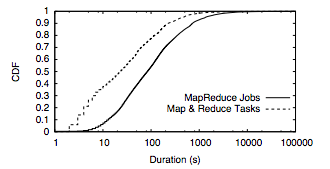
\includegraphics[scale=0.6]{./figures/mesos_workload}
  \label{fig:mesos_workload}
\end{figure}

\begin{itemize}
	\item {\bf Typical workloads in ``Data Warehouse'' systems}
	\begin{itemize}
		\item Heterogeneous MapReduce jobs, {\it production} and {\it ad-hoc} queries
		\item Large scale machine learning
		\item SQL-like queries
	\end{itemize}
\end{itemize}
\end{frame}

%%%%%%%%%%%%%%%%%%%%%%%%%%%%%%%%%%%%%%%%%%%%%%%%%%%%%%%%%%%%%%%%%%%%%%%%%%%%%%%
\subsection{Architecture}
%%%%%%%%%%%%%%%%%%%%%%%%%%%%%%%%%%%%%%%%%%%%%%%%%%%%%%%%%%%%%%%%%%%%%%%%%%%%%%%
\begin{frame}
 \begin{colorblock}{blue}{lightblue}{ }
    \Large \textbf{Architecture}
  \end{colorblock}
\end{frame}

\begin{frame}
\frametitle{Design Philosophy}
\begin{itemize}
	\item {\bf Data center operating system}
	\begin{itemize}
		\item Scalable and resilient core exposing low-level interfaces 
		\item High-level libraries for common functionalities
	\end{itemize}

	\item {\bf Minimal interface to support resource sharing}
	\begin{itemize}
		\item Mesos manages cluster resources
		\item Frameworks control task scheduling and execution
	\end{itemize}

	\item {\bf Benefits of two-level approach}
	\begin{itemize}
		\item Frameworks are independent and can support diverse scheduling requirements
		\item Mesos is kept simple, minimizing the rate of change to the system
	\end{itemize}
\end{itemize}
\end{frame}

\begin{frame}
\frametitle{Architecture Overview}
\begin{figure}[h]
  \centering
  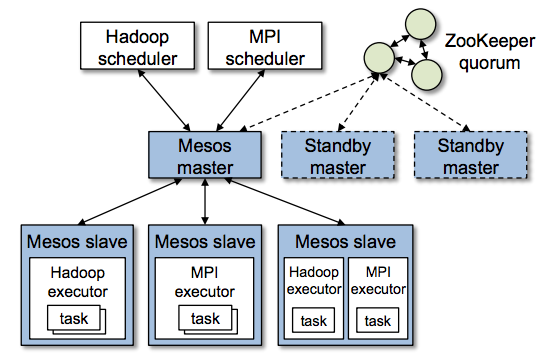
\includegraphics[scale=0.6]{./figures/mesos_arch_overview}
  \label{fig:mesos_arch_overview}
\end{figure}
\end{frame}

\begin{frame}
\frametitle{Architecture Overview}
{\bf The Mesos Master}
\begin{itemize}
	\item Uses {\bf Resource Offers} to implement fine-grained sharing
	\item Collects resource utilization from slaves
	\item Resource offer: list of free resources on multiple slaves
\end{itemize}

\begin{block}{First-level Scheduling}
\begin{itemize}
	\item Master decides how many resources to offer a framework
	\item Implements a cluster-wide allocation policy:
	\begin{itemize}
		\item Fair Sharing
		\item Priority based
	\end{itemize}
\end{itemize}
\end{block}
\end{frame}

\begin{frame}
\frametitle{Architecture Overview}
{\bf Mesos Frameworks}
\begin{itemize}
	\item Framework {\bf scheduler}
	\begin{itemize}
		\item Registers to the master
		\item Selects {\bf which offer to accept}
		\item Prepares a description of the tasks to launch on accepted resources
	\end{itemize}	
	\item Framework {\bf executor}
	\begin{itemize}
		\item Launched on Mesos slaves executing on accepted resources
		\item Takes care of running the framework's tasks
	\end{itemize}
\end{itemize}
\begin{block}{Second-level Scheduling}
\begin{itemize}
	\item One framework scheduler per application
	\item Framework decides how to execute an application (a job) and its tasks
	\item {\bf NOTE:} The actual task execution is requested by the master
\end{itemize}
\end{block}
\end{frame}

\begin{frame}
\frametitle{Resource Offer Example}
\begin{figure}[h]
  \centering
  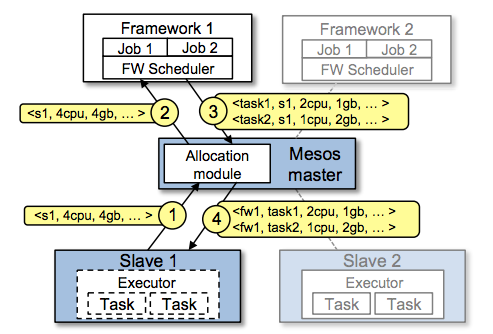
\includegraphics[scale=0.6]{./figures/mesos_arch_example}
  \label{fig:mesos_arch_example}
\end{figure}
\end{frame}

\begin{frame}
\frametitle{Consequences of the Mesos Architecture}
\begin{itemize}
	\item {\bf Mesos makes no assumptions on Framework requirements}
	\begin{itemize}
		\item This is unlike other approaches, which requires the cluster scheduler to understand application constraints
		\item This does not mean that users are not required to express their applications' constraints
	\end{itemize}

	\item {\bf Rejecting offers}
	\begin{itemize}
		\item It is the framework that decides to reject a resource offer that does not satisfy application constraints
		\item Frameworks can {\bf wait} for offers to satisfy constraints
	\end{itemize}
\end{itemize}

\begin{block}{Arbitrary and complex resource constraints}
\begin{itemize}
	\item Delegate logic and control to individual frameworks
	\item Mesos also implements {\bf filters} to optimize the resource offer mechanism
\end{itemize}
\end{block}
\end{frame}

\begin{frame}
\frametitle{Resource Allocation}
\begin{itemize}
	\item {\bf Pluggable allocation module}
	\begin{itemize}
		\item Max-min Fairness
		\item Strict priority
	\end{itemize}
	\item {\bf Fundamental assumption}
	\begin{itemize}
		\item Tasks are short
		\item[$\to$] Mesos only reallocates resources when tasks finish
	\end{itemize}
	\item {\bf Example}
	\begin{itemize}
		\item Assume a Framework's share is 10\% of the cluster
		\item It needs to wait $~10$\% of the mean task length to receive its share
	\end{itemize}
\end{itemize}
\end{frame}

\begin{frame}
\frametitle{Resource Revocation}
\begin{itemize}
	\item {\bf Short vs. long lived tasks}
	\begin{itemize}
		\item Some jobs (e.g. streaming) may have long tasks
		\item In this case, Mesos can {\bf Kill} running tasks
	\end{itemize}
	\item {\bf Preemption primitives}
	\begin{itemize}
		\item Require knowledge about potential resource usage by frameworks
		\item Killing might be wasteful, although not critical (e.g. MapReduce)
		\item Some applications (e.g. MPI) might be harmed
	\end{itemize}
	\item {\bf Guaranteed allocation}
	\begin{itemize}
		\item Minimum set of resources granted to a framework
		\item If below guaranteed allocation $\to$ never kill tasks
		\item If above guaranteed allocation $\to$ kill any tasks
	\end{itemize}
\end{itemize}
\end{frame}

\begin{frame}
\frametitle{Performance Isolation}
\begin{itemize}
	\item {\bf Isolation between executors on the same slave}
	\begin{itemize}
		\item Achieved through low-level OS primitives
		\item Pluggable isolation modules to support a variety of OS
	\end{itemize}
	\item {\bf Currently supported mechanisms}
	\begin{itemize}
		\item Limit CPU, memory, network and I/O bandwidth of a process tree
		\item Linux Containers and Solaris Cages
	\end{itemize}
	\item {\bf Advantages and limitations}
	\begin{itemize}
		\item Better isolation than current approach, process-based
		\item Fine grained isolation is not yet fully functional
	\end{itemize}
\end{itemize}
\end{frame}

\begin{frame}
\frametitle{Mesos Scalability}
\begin{itemize}
	\item {\bf Filter mechanism}
	\begin{itemize}
		\item Short-circuit the rejection process, avoids unnecessary communication
		\item Filter type 1: restrict which slave machines to use
		\item Filter type 2: check resource availability on slaves
	\end{itemize}
	\item {\bf Incentives to speed-up the resource offer mechanism}
	\begin{itemize}
		\item Mesos counts offers to a framework toward its allocation
		\item Frameworks have to answer and/or filter as quickly as possible
	\end{itemize}
	\item {\bf Rescinding offers}
	\begin{itemize}
		\item Mesos can decide to invalidate an offer to a framework
		\item This avoids blocking and misbehavior
	\end{itemize}
\end{itemize}
\end{frame}

\begin{frame}
\frametitle{Mesos Fault Tolerance}
\begin{itemize}
	\item {\bf Master designed with {\it Soft State}}
	\begin{itemize}
		\item List of active slaves
		\item List of registered frameworks
		\item List of running tasks
	\end{itemize}
	\item {\bf Multiple masters in a hot-standby mode}
	\begin{itemize}
		\item Leader election through Zookeeper
		\item Upon failure detection new master is elected
		\item Slaves and executors help populating the new master's state
	\end{itemize}
	\item {\bf Helping frameworks to tolerate failure}
	\begin{itemize}
		\item Master sends ``health reports'' to framework schedulers
		\item Master allows multiple schedulers for a single framework
	\end{itemize}
\end{itemize}
\end{frame}

%%%%%%%%%%%%%%%%%%%%%%%%%%%%%%%%%%%%%%%%%%%%%%%%%%%%%%%%%%%%%%%%%%%%%%%%%%%%%%%
\subsection{Mesos Behavior}
%%%%%%%%%%%%%%%%%%%%%%%%%%%%%%%%%%%%%%%%%%%%%%%%%%%%%%%%%%%%%%%%%%%%%%%%%%%%%%%
\begin{frame}
 \begin{colorblock}{blue}{lightblue}{ }
    \Large \textbf{System behavior: a very rough Mesos ``model''}
  \end{colorblock}
\end{frame}

\begin{frame}
\frametitle{Overview: Mesos in a nutshell}
\begin{itemize}
	\item {\bf Ideal workloads for Mesos}
	\begin{itemize}
		\item Elastic frameworks, supporting scaling up and down seamlessly
		\item Task durations are homogeneous (and short)
		\item No strict preference over cluster nodes
	\end{itemize}
	\item {\bf Frameworks with cluster node preferences}
	\begin{itemize}
		\item Assume frameworks prefer different (and possibly disjoint) nodes
		\item Mesos can emulate a centralized scheduler
		\item Cluster and Framework wide fair resource sharing
	\end{itemize}
	\item {\bf Heterogeneous task durations}
	\begin{itemize}
		\item Mesos can handly coexisting short and long lived tasks
		\item Performance degradation is acceptable
	\end{itemize}
\end{itemize}
\end{frame}

\begin{frame}
\frametitle{Definitions}
\begin{itemize}
	\item {\bf Workload characterization}
	\begin{itemize}
		\item {\it Elasticity:} elastic workloads can use resources as soon as they are acquired, and releases them as soon as tasks finish; in contrast, rigid frameworks (e.g. MPI) can only start a job when {\bf all} resources have been acquired, and do not work well with scaling
		\item {\it Task runtime distribution:} both homogeneous and not
	\end{itemize}
	\item {\bf Resource characterization}
	\begin{itemize}
		\item {\it Mandatory:} resource that a framework {\bf must} acquire to work. Assumption: mandatory resources $<$ guaranteed share
		\item {\it Preferred:} resources that a framework {\bf should} acquire to achieve better performance, but are not necessary for the job to work
	\end{itemize}
\end{itemize}
\end{frame}

\begin{frame}
\frametitle{Performance Metrics}
\begin{itemize}
	\item {\bf Performance metrics}
	\begin{itemize}
		\item {\it Framework ramp-up time:} time it takes a new framework to achieve its fair share
		\item {\it Job completion time:} time it takes a job to complete. Assume one job per framework
		\item {\it System utilization:} total cluster resource utilization, with focus on CPU and memory
	\end{itemize}
\end{itemize}
\end{frame}

\begin{frame}
\frametitle{Homogeneous Tasks}
\begin{itemize}
	\item Cluster with $n$ slots and a framework $f$ entitled with $k$ slots
	\item Task runtime distribution: uniform and exponential
	\item Mean task duration $T$
	\item Job duration: $\beta k T$
	\item[$\to$] If $f$ has $k$ slots, then job duration is $\beta T$
\end{itemize}
\begin{figure}[h]
  \centering
  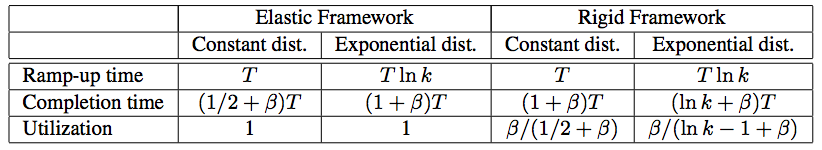
\includegraphics[scale=0.4]{./figures/mesos_model}
  \label{fig:mesos_arch_example}
\end{figure}
\end{frame}

\begin{frame}
\frametitle{Placement preferences}
Consider two cases:
\begin{itemize}
	\item {\bf There exist a configuration satisfying all frameworks constraints}
	\begin{itemize}
		\item The system will eventually converge to the state in which the optimal allocation is achieved, and this in at most one $T$ interval
	\end{itemize}
	\item {\bf No such allocation exists, e.g. demand is larger than supply}
	\begin{itemize}
		\item {\bf Lottery Scheduling} to achieve a {\bf weighted fair allocation}
		\item Mesos offers a slot to framework $i$ with probability 
		$$ \frac{s_i}{\sum_{i=1}^{m}s_i} $$
		\item where $s_i$ is framework's $i$ {\bf intended} allocation, and $m$ is the total number of frameworks registered to Mesos
	\end{itemize}
\end{itemize}
\end{frame}

\begin{frame}
\frametitle{Heterogeneous Tasks}
\begin{itemize}
	\item {\bf Assumptions}
	\begin{itemize}
		\item Workloads with tasks that are either long or short
		\item Mean duration of long task is longer than short ones
	\end{itemize}
	\item {\bf Worst case scenario}
	\begin{itemize}
		\item All nodes required by a ``short job'' are filled with long tasks, which means it has to wait for a long time
	\end{itemize}
	\item {\bf How likely is the worst case?}
	\begin{itemize}
		\item Assume $\phi < 1$, where $\phi$ fraction of long tasks
		\item Assume a cluster with $S$ available slots per node
		\item[$\to$] Probability for a node to be filled with long tasks is $\phi^S$
		\item $S=8$ and $\phi = 0.5$ gives a 0.4\% chance 
	\end{itemize}
\end{itemize}
\end{frame}

\begin{frame}
\frametitle{Limitations of Distributed Scheduling}
\begin{itemize}
	\item {\bf Fragmentation}
	\begin{itemize}
		\item Provokes under utilization of system resources
		\item Distributed collection of frameworks might not achieve the same ``packing'' quality of a centralized scheduler
		\item[$\to$] This is mitigated by having clusters of ``big'' nodes (many CPUs, many cores) running ``small'' tasks
	\end{itemize}
	\item {\bf Starvation}
	\begin{itemize}
		\item Large jobs may wait indefinitely for slots to become free
		\item Small tasks from small jobs might monopolize the cluster
		\item[$\to$] This is mitigated by a {\it minimum offer size} mechanism
	\end{itemize}
\end{itemize}
\end{frame}

%%%%%%%%%%%%%%%%%%%%%%%%%%%%%%%%%%%%%%%%%%%%%%%%%%%%%%%%%%%%%%%%%%%%%%%%%%%%%%%
\subsection{Mesos Performance}
%%%%%%%%%%%%%%%%%%%%%%%%%%%%%%%%%%%%%%%%%%%%%%%%%%%%%%%%%%%%%%%%%%%%%%%%%%%%%%%
\begin{frame}
 \begin{colorblock}{blue}{lightblue}{ }
    \Large \textbf{Experimental Mesos Performance Evaluation}
  \end{colorblock}
\end{frame}

\begin{frame}
\frametitle{Resource Allocation}
\begin{figure}[h]
  \centering
  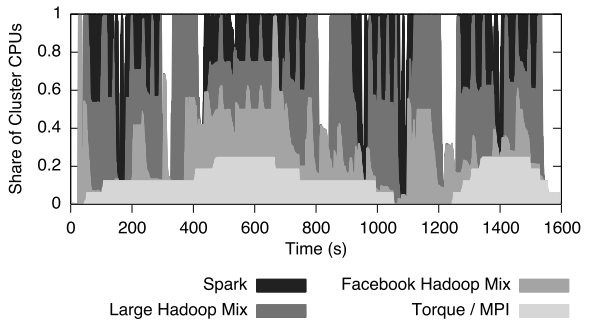
\includegraphics[scale=0.55]{./figures/mesos_perf_fm}
  \label{fig:mesos_perf_ru}
\end{figure}
\end{frame}

\begin{frame}
\frametitle{Resource Utilization}
\begin{figure}[h]
  \centering
  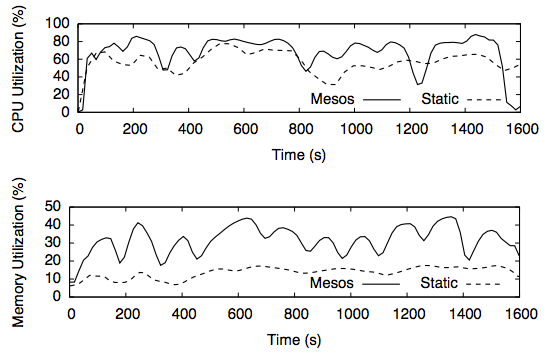
\includegraphics[scale=0.6]{./figures/mesos_perf_ru}
  \label{fig:mesos_perf_ru}
\end{figure}
\end{frame}

\begin{frame}
\frametitle{Data Locality}
\begin{figure}[h]
  \centering
  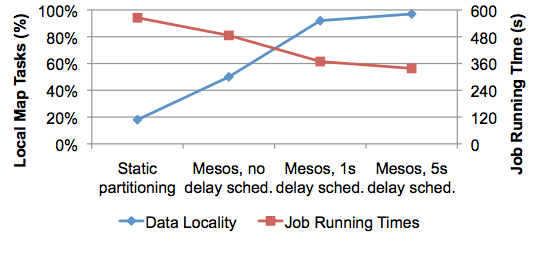
\includegraphics[scale=0.6]{./figures/mesos_perf_dl}
  \label{fig:mesos_perf_dl}
\end{figure}
\end{frame}
